\documentclass[a4paper,14pt]{extreport}

\usepackage[T2A]{fontenc}
\usepackage[utf8]{inputenc}
\usepackage{totcount}

\usepackage[english,russian]{babel}

\usepackage{amsthm}

\usepackage{hyperref}

\usepackage[dvips]{graphicx}
\usepackage{caption}
\usepackage{subcaption}
\graphicspath{{images/eps/}}

\usepackage{titlesec}
\usepackage{listings}
\usepackage{indentfirst}
\usepackage{cite}


\usepackage{geometry}
\geometry{left=3cm}
\geometry{right=1cm}
\geometry{top=1.5cm}
\geometry{bottom=2cm}



\renewcommand{\baselinestretch}{1.2}

\lstset{numbers=left,
        frame=single,
        breaklines=true,
        breakatwhitespace=true,
        basicstyle=\ttfamily\small}

\begin{document}

\makeatletter
\renewcommand{\@biblabel}[1]{#1.}
\makeatother

\titleformat{\chapter}[hang]{\huge\bfseries}{\thechapter. }{0pt}{\hyphenpenalty=10000\huge\bfseries}

\renewcommand{\theenumi}{\arabic{enumi}}
\renewcommand{\labelenumi}{\arabic{enumi}}
\renewcommand{\theenumii}{.\arabic{enumii}}
\renewcommand{\labelenumii}{\arabic{enumi}.\arabic{enumii}}
\renewcommand{\theenumiii}{.\arabic{enumiii}}
\renewcommand{\labelenumiii}{\arabic{enumi}.\arabic{enumii}.\arabic{enumiii}}

\newtotcounter{figurecnt}
\def\oldfig{} \let\oldfig=\figure
\def\figure{\stepcounter{figurecnt}\oldfig}
%òàáëèö (only longtable)
\newtotcounter{tablecnt}
\def\oldtab{} \let\oldtab=\table
\def\table{\stepcounter{tablecnt}\oldtab}

\newtotcounter{bibitemcnt}
\renewcommand{\citeform}[1]{%
\ifnum#1>\totvalue{bibitem}%
{\setcounter{bibitem}{#1} }\fi%
#1%
}

\regtotcounter{page}

\def\formbytotal#1#2#3#4#5{%
    \newcount\c
    \c \totvalue{#1}\relax
    \newcount\last
    \newcount\pnul
    \last \c\relax
    \divide \last 10
    \pnul \last\relax
    \divide\pnul 10
    \multiply \pnul-10
    \advance \pnul\last
    \multiply \last-10
    \advance \last\c
    \total{#1}~#2%
    \ifnum\pnul=1#5\else%
        \ifcase\last#5\or#3\or#4\or#4\or#4\else#5\fi
    \fi
}

\renewcommand{\lstlistingname}{Листинг}
\renewcommand\contentsname{Содержание}

\newtheorem{Def}{Определение}[section]

\setcounter{page}{2}

\chapter*{Реферат}

	%TODO: разберись, как пишется: "онлайн среда разработки" - с дефисом или без 
	Дипломный проект изложен на~\formbytotal{page}{страниц}{е}{ах}{ах}, содержит \formbytotal{tablecnt}{таблиц}{у}{ы}{}, \formbytotal{figurecnt}{рисун}{ок}{ка}{ков}, 11 источников.

	Целью данного проекта является создание новой версии онлайн среды разработки для языка Котлин.

	В результате данного проекта было создано интернет-приложение с масштабируемой архитектурой, располагающееся по адресу\\ http://try.kotlinlang.org/. 
	
	Работа состоит из четырёх глав, введения и заключения.
Во введении в краткой форме объясняются причины возникновения необходимости выполнения такого рода работы, цель и задачи проекта.
В первой главе проводится краткий обзор предметной области.
Во второй главе описывается устройство приложения.
В третьей главе приведено описание системы публикации приложения с учётом масштабируемости его архитектуры.
Четвёртая глава посвящена тестированию приложения.
В заключении подводятся итоги и описываются возможные направления дальнейших работ.

\clearpage

\tableofcontents

\chapter*{Введение}
\addcontentsline{toc}{chapter}{Введение}  

	На ранних этапах развития интернета каждая web-страница доставлялась клиенту как статический документ, а интерактивность достигалась за счёт последовательности различных страниц. У такого подхода был недостаток~--- при каждом значительном изменении веб-страницы требовалось обратиться к серверу и перезагрузить эту страницу целиком. 

	В 1995 году компания Netscape выпустила язык программирования 
Java\-Script, который исполнялся на стороне клиента и позволял выполнять ряд задач, не обращаясь при этом к серверу. Вторым важным моментом было развитие AJAX-запросов~--- запросов к серверу, которые не требовали перезагрузки страницы. 
	
	Развитие этих двух технологий привело к появлению интернет-приложе\-ний~--- интерактивных web-сайтов, которые могут целиком располагаться на одной странице,  взаимодействуя с пользователем при помощи JavaScript кода, а с сервером при помощи AJAX запросов. На сегодняшний день такой формат сайтов очень популярен, т.к. он позволяет намного больше, чем последовательность интернет-страниц, например, писать браузерные игры, отображать карту и т.д.
	
	Одним из многочисленных типов интернет-приложений являются онлайн среды разработки~--- сайты, которые позволяют запустить код на том или ином языке в браузере. Они позволяют пользователям познакомиться с новым для них языком, а также предоставляют простой способ демонстрировать другим пользователям свой код (например, сайт jsfiddle почти всегда используется для публикации кода в качестве иллюстрации к ответам на вопросы, касающиеся HTML/CSS/JavaScript).
	
	Подобные приложения есть почти для всех распространённых языков программирования, например:
\begin{itemize}
	\item http://www.simplyscala.com/ - приложение, позволяющее запускать код на языке scala. 
	\item http://try.ceylon-lang.org/ - приложение, позволяющее запускать код на языке ceylon.
	\item http://www.tutorialspoint.com/ - приложение, позволяющее запускать код на большом количестве разнообразных языков программирования.
	\item \dots
\end{itemize}


	Онлайн-среда разработки для языка Котлин \cite{project_kotlin} называется Kotlin Web Demo. Данное приложение учитывает специфику  языка и позволяет как запускать код внутри виртуальной машины Java, которая располагается на сервере, так и транслировать код в JavaScript и исполнять его в браузере. Также в этом приложении есть подсветка синтаксиса, подсветка ошибок и автодополнение кода, что значительно упрощает процесс его написания.
	
	%TODO: разобраться со временами
	Недостатком данной среды разработки является исполнение всех запросов внутри одного сервера. Такая архитектура приложения является самой простой, однако при увеличении нагрузки приложение утрачивает работоспособность. Подобная ситуация наблюдалась при публикации Kotlin Web Demo и может повториться, например, при публикации новой версии Котлина.
	
	
	Вторым существенным недостатком была необходимость размещения  исполняемого кода  пользовательского примера внутри одного файла. Это не было проблемой само по себе, т.к. основная цель~--- дать пользователю познакомиться с языком, а не предоставить ему возможность писать большие программы, однако это стало проблемой, когда возникла идея использовать Kotlin Web Demo для запуска программ-заданий. Каждое такое задание требует от пользователя написать код на Котлине, который решает определённую задачу, а потом при помощи тестов проверяет, что код решает задачу корректно. Для реализации этого требовалось разделить код на файл с тестами и файл с пользовательским кодом, что и привело к возникновению вышеописанной проблемы.
	
	
	\underline{Целью} данного проекта является создание новой версии онлайн среды разработки.
	
	Основные \underline{задачи}, решаемые в работе:
	\begin{itemize}
		\item { \bf Создание автоматически масштабируемой архитектуры приложения} -- для работоспособности сервера в случае резкого увеличения нагрузки.
		\item { \bf Поддержка многофайловых проектов и JUnit тестов} -- для запуска программ-заданий.
	\end{itemize}
		



\chapter{Обзор предметной области}
\section{Технологии, использующиеся в приложении}
	Данный проект, как и другие интернет-приложения,  состоит из клиентской и серверной части. В этой главе даётся краткий обзор тех технологий и языков программирования, которые использовались для написания обоих частей.
\subsection{Клиентская часть}
	Для написания клиентской части используются следующие технологии и языки программирования:
\begin{itemize}
	\item \textbf{HTML/CSS} -- стандартные технологии веб программирования, используемые для верстки веб приложения.
	\item \textbf{JavaScript} -- высокоуровневый динамический язык программирования, который используется в основном для клиентской части интернет-приложений. Позволяет взаимодействовать с пользователем, изменять видимый пользователю документ, отправлять AJAX-запросы серверу. JavaScript позволяет писать как в функциональном, так и в объектно-ориентированном стиле, однако используемое в языке ``прототипное наследование'' обусловливает отличия в работе с объектами по сравнению с традиционными языками, использующими классы.
	\item \textbf{Jquery} -- распространённая библиотека для JavaScript, которая добавляет простой и достаточно удобный интерфейс для отправки запросов к серверу, обработки событий, взаимодействия с DOM-деревом и многого другого.
	\item \textbf{Jquery UI} -- библиотека, основанная на JQuery. Предоставляет интерфейс для создания различных элементов сайта, таких как диалоги, вкладки, кнопки и.т.д.
	\item \textbf{CodeMirror} -- редактор кода, написанный на языке JavaScript. Данный редактор является стандартом де-факто для тех приложений, в которых требуется редактировать/демонстрировать код. На данный момент поддерживает более 100 языков и обладает достаточно простым интерфейсом, позволяющим легко поддержать любой новый язык. Так же он обладает системой плагинов, которая позволяет его персонализировать, добавляя те возможности, которые вас интересуют (например, поиск, автодополнение, подсветка текущей строки и.т.д.)
	\item \textbf{Котлин} -- статически типизированный объектно-ориентированный язык программирования, который может быть скомпилирован в JavaScript. Котлин, как и JavaScript, позволяет писать не только в объектно-ориентированном, но и в функциональном стиле. Так же в Котлине создан ряд абстракций (аннотация native, dynamic тип и др.), которые позволяют взаимодействовать с кодом на JavaScript. Благодаря этому, в большинстве случаев, код, написанный на JavaScript, достаточно легко транслируется в код на Котлине. 
\end{itemize}

\subsection{Сервер}
	Серверная часть приложения написана на языке Java. В качестве сервера используется Tomcat.

	\textbf{Tomcat} -- сервер, написанный на языке Java и разрабатываемый компанией Apache. Tomcat реализует ряд спецификаций языка Java, таких как Java Servlet и JavaServer Pages. Для обработки запросов, приходящих на сервер, томкат использует отдельные потоки, количество которых может регулироваться в настройках сервера. 
	
	Также в серверной части приложения используется \textbf{MySql} -- реляционная база данных.
	
\section{Технологии, использующиеся для тестирования}
	Тестирование интернет-приложения, как правило, состоит из нескольких частей -- тестирования клиентского кода, тестирование серверного кода, а так же тестирование поведения сервера при большом количестве запросов (нагрузочное тестирование).
	
	Для проведения этих частей тестирования в данном проекте используются следующие технологии:
	\begin{itemize}
\item Тестирование серверного кода:
	\begin{itemize}
		\item \textbf{JUnit} -- распространённая библиотека для написания unit-тестов на языке Java.
	\end{itemize}
\item Нагрузочное тестирование:
	\begin{itemize}
		\item \textbf{JMeter} -- графическое Java приложение, предназначенное для написания нагрузочного тестирования и измерения производительности при нагрузочном тестировании. Данное приложение позволяет отправлять различного рода запросы (нас интересуют HTTP запросы) и анализировать производительность сервера при обработке этих запросов.
	\end{itemize}
\item Тестирование клиентского кода:
\begin{itemize}
	\item \textbf{nodejs} -- платформа, позволяющая запускать код на языке JavaScript. Обычно используется для создания серверов и сетевых приложений. В данном проекте используется для запуска karma.
	\item \textbf{karma} -- приложение для запуска тестов на языке JavaScript. Может исполнять тесты во всех популярных браузерах(Google Chrome, Opera, Safari \dots), а так же внутри phantomjs. Это приложение само написано на JavaScript и предназначено для запуска при помощи nodejs.
	\item \textbf{phantomjs} -- браузер без графического интерфейса, созданный для автоматического тестирования веб приложений. Данный браузер основан на платформе WebKit, что делает его похожим по поведению на такие браузеры как Chrome и Safari.
	\item \textbf{qunit} -- распространённая библиотека для написания unit-тестов на языке JavaScript.
\end{itemize}
\end{itemize}

\section{Публикация интернет-приложений}
В данной главе освещаются технологии, используемые нами для публикации приложения.
\subsection{Amazon Web Services}
	Amazon Web Service -- это набор сервисов, предоставляемый компанией Amazon. Данные сервисы предоставляют возможность создания масштабируемой инфраструктуры на машинном уровне и состоят из следущих компонент:
\begin{itemize}
	\item \textbf{Amazon EC2 instance} -- пожалуй, один из основных элементов всей инфраструктуры. EC2 instance -- это компьютер, предоставляемый амазоном, параметры которого можно выбирать при старте, основываясь на требованиях к данному компьютеру. В зависимости от параметров меняется и стоимость данного компьютера.
	\item \textbf{Amazon Machine Image (AMI)} -- снимок памяти компьютера, необходим для того, чтобы запустить EC2 instance. Существует большое количество публичных AMI, которые, как правило, содержат операционную систему (например, для запуска EC2 instance с Ubuntu необходимо найти идентификатор AMI содержащего Ubuntu  и указать его при старте машины). Так же пользователь может создать свой AMI, содержащий специфичную для данной задачи информацию.
	\item \textbf{Launch Configuration} -- конфигурация, которая содержит все данные, необходимые для запуска EC2 instance, такие как: 
	\begin{itemize}
		\item Instance type -- определяет мощность CPU, количество памяти и другие подобные параметры  EC2 instance.
		\item AMI ID -- идентификатор AMI
		\item User Data -- скрипт, который будет исполнен после запуска машины. Позволяет автоматизировать запуск машины.
		\item ...
	\end{itemize}
	\item \textbf{Cloud Watch Monitoring} -- сервис, который собирает и хранит информацию о других сервисах, например, для каждого EC2 instance хранятся: 
	\begin{itemize}
		\item Потребление CPU
		\item Количество операций чтения/записи на диск
		\item \dots
	\end{itemize}
	Вся эта информация доступна через веб интерфейс Amazon. %ссылка на какую-нибудь картинку%.
	\item \textbf{Cloud Watch Monitoring Alarm} -- настраиваемые события внутри Cloud Watch Monitoring. Например, ``среднее потребление CPU у EC2 instnance более 80\% в течении 5 минут''. Может использоваться как для оповещения администратора, так и для управления масштабированием
	\item \textbf{Auto Scaling Group (ASG)} -- система, позволяющая запускать заданное количество EC2 instance. Их количество может выставляться как вручную, так и на основании Cloud Watch Monitoring Alarmsdamnaleto-ов.
	\item \textbf{Elastic Load Balancer (ELB)} -- балансировщик нагрузки. Распределяет приходящие на него HTTP-запросы между компьютерами, которые к нему подключены.
\end{itemize}


Кроме перечисленных выше сервисов нами использовались сервисы, связанные с безопасностью, доменными именами и.т.д., однако они являются техническими и их описание не представляет особого интереса.

\subsection{Cхема работы автоматического масштабирования в AWS}
	Перечисленные выше сервисы, как правило, не используются сами по себе, а собираются в большую систему. В данном параграфе я покажу как в общем из описанных выше сервисов получается автоматически масштабируемая система.
	
	Схема работы автоматического масштабирования приведена на рис.\ref{fig:aws_autoscaling}.
	
\begin{figure}[h]
    \centering
    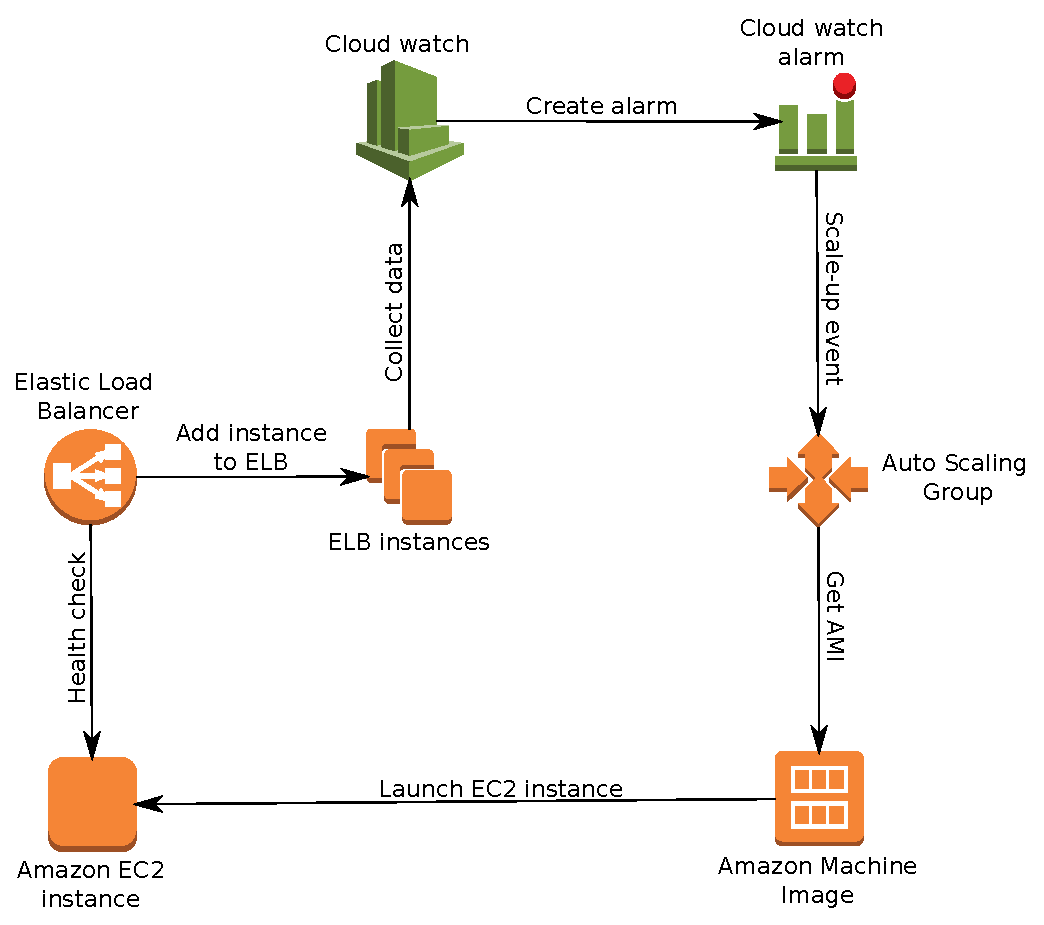
\includegraphics[scale=0.8]{amazon_scale_up.eps} 
    \caption{Принципиальная схема работы автоматического масштабирования в AWS}
    \label{fig:aws_autoscaling}
\end{figure}
	Рассмотрим как это всё работает начиная с процесса создания. Первым создаётся балансировщик нагрузки (ELB). В начале к нему не прикреплен ни один компьютер, поэтому, если на него приходит запрос, то он просто отвечает HTTP статусом 503 (сервис недоступен).
	
	Далее создаётся система автоматического масштабирования (ASG). При её создании необходимо иметь конфигурацию (Launch Configuration), основываясь на которой она будет запускать новые компьютеры в случае надобности. Также нужно создать события (Cloud Watch Alarms), которые будут послать сигналы для увеличения/уменьшения количества машин в системе масштабирования. Каждое из этих событий следит за потреблением одного из ресурсов, например, потреблением CPU и позволяет отреагировать на то, что мы данный ресурс исчерпываем (нужно запустить больше машин), либо у нас его слишком много (нужно остановить несколько машин).
	
	После создания система, используя заданную конфигурацию, автоматически поднимает минимальное количество машин (параметр, передающийся при запуске) и подключает их к ELB. Балансировщик нагрузки выполняет проверку того, что переданные ему машины работоспособны (определённым образом отвечают на определённый запрос) и, как только убеждается в их работоспособности, начинает отправлять туда запросы.
	
	Дальнейшее масштабирование происходит на основе данных в системе мониторинга (Cloud Watch Monitoring). Данные, полученные с запущенных машин, сравниваются с настроенными нами событиями и на основании их система масштабирования автоматически  запускает (аналогично предыдущему пункту), либо останавливает компьютеры.
	
	Кроме описанного выше случая компьютер может быть остановлен если он в какой-то момент не пройдёт проверку работоспособности от ELB. В такой ситуации система масштабирования попытается поднять новую машину на замену неработоспособной. Это позволяет автоматически восстанавливать систему если что-то произошло на одном из компьютеров, однако может привести к неприятным последствиям, которые будут освещены в главе \ref{}.

\subsection{Docker}

	Docker - технология виртуализации, которая последнее время набирает всё большую популярность среди разработчиков. 
	
	Отличие докера от виртуальных машин, которые также являются способом виртуализации, заключается в основном в легковесности. Каждая виртуальная машина должна кроме приложения (которое может иметь размер в несколько мегабайт) подгружать ещё и окружение (которое может иметь размер в несколько гигабайт). В отличии от этого докер-контейнер содержит только приложение и его зависимости и запускается в изолированном процессе в пространстве пользователя, разделяя ядро с другими контейнерами.
\begin{figure}[h]
	\centering
	\begin{subfigure}[b]{.5\textwidth}
  		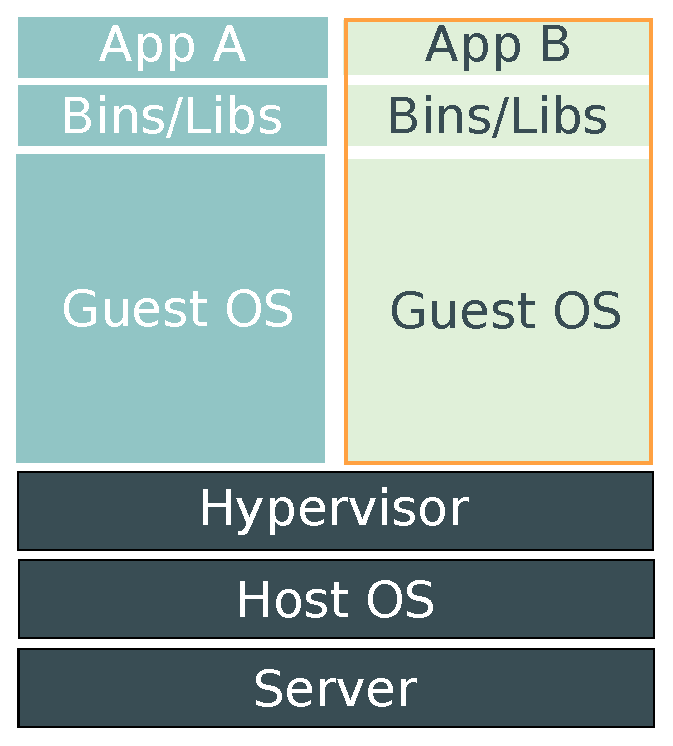
\includegraphics[width=.9\linewidth]{vm_scheme}
  		\caption{Virtual Machines}
  		\label{fig:sub1}
	\end{subfigure}%
	\begin{subfigure}[b]{.5\textwidth}
  		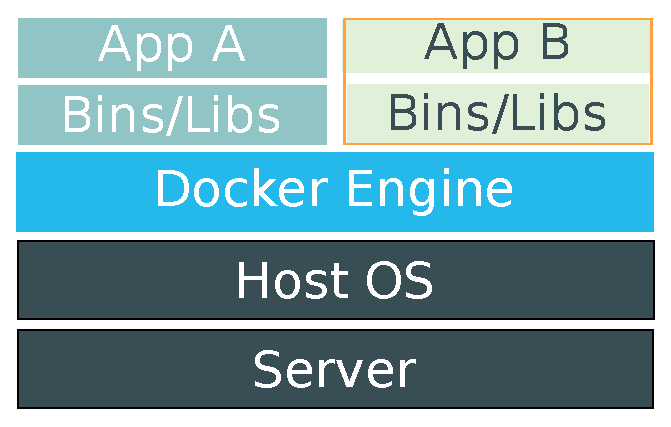
\includegraphics[width=.9\linewidth]{docker_scheme}
  		\caption{Docker}
  		\label{fig:sub2}
	\end{subfigure}
	\caption{Сравнение виртуализации при помощи виртуальных машин и при помощи докер контейнеров}
	\label{fig:test}
\end{figure}

	Каждый докер-контейнер основан докер-образе. Докер-образ это шаблон, по которому мы можем запускать контейнеры. В нём мы можем указать операционную систему, которую мы хотим использовать, установить необходимое окружение, и.т.д. Образы можно как собирать, основываясь на файле с инструкциями, так и скачивать с хранилищ.
	
	Каждый образ состоит из слоёв. Слой это состояние контейнера после того, как мы выполнили очередную команду. Такая структура позволяет нам при обновлениях образа вместо обновления всего приложения обновить только изменившиеся слои.
\subsection{Операционная система}
\begin{itemize}

	\item {\bf CoreOS} - операционная система, предназначенная для запуска всего внутри контейнеров Linux, например, при помощи докера, о котором шла речь в предыдущем пункте. В связи с такой специфической направленностью в CoreOS отсутствуют почти все привычные для пользователя Linux пакеты и программы (yum, apt-get, wget \dots), грубо говоря, там есть только докер.
	
	\item {\bf systemd} - демон инициализации других демонов в Linux. Systemd позволяет описывать сервис, который мы собираемся запустить, в текстовом виде. Ниже приведён пример файла сервиса, который запускает докер контейнер.
\begin{lstlisting}
[Unit]
Description=My Service
Requires=docker.service
After=docker.service

[Service]	
ExecStart=/usr/bin/docker run busybox /bin/sh -c "while true; do echo Hello World; sleep 1; done"

[Install]
WantedBy=multi-user.target
\end{lstlisting}
\end{itemize}
	Кроме запуска systemd следит за работоспособностью запущенных сервисов и, если какой-то из них возвращает ошибку, перезапускает его (если не настроить обратное).
\section{Обновление приложений}
Существует множество различных способов обновления интернет-приложения в зависимости от требований к нему. Самыми простыми из них являются:
\begin{itemize}
	\item {\bf Выключать приложение для обновления.} Данный подход является наиболее простым, однако обладает рядом очевидных недостатков, а именно:
	\begin{itemize}
		\item Приложение недоступно в течении обновления.
		\item Невозможно протестировать обновлённое приложение перед его публикацией.
		\item Сложно восстановить работоспособность приложения при неудачном обновлении.
	\end{itemize}
	\item {\bf Создавать копию приложения вместе с инфраструктурой.} При таком подходе обновляется то приложение, которое на данный момент не принимает запросы от пользователя. После обновления все запросы начинают отправляться на новую версию приложения, а старая версия становится неактивной до следующего обновления. Недостатком такого подхода является необходимость создания копии всей инфраструктуры.
	\item {\bf Создавать копию приложения (Blue-Green deployment).} Данный подход известен  как аналогичен предыдущему, но в нём неактивное приложение располагается внутри той же инфраструктуры, что и активное. Недостатки данного подхода будут описаны подробней в главе \ref{sec}
\end{itemize}
\chapter{Устройство приложения}
	Серверная часть данного проекта состоит из внешнего сервера, внутренних серверов и базы данных, см рис.\ref{fig:app_schema}.
\begin{figure}[h]
	\label{app_schema}
	\begin{center}
	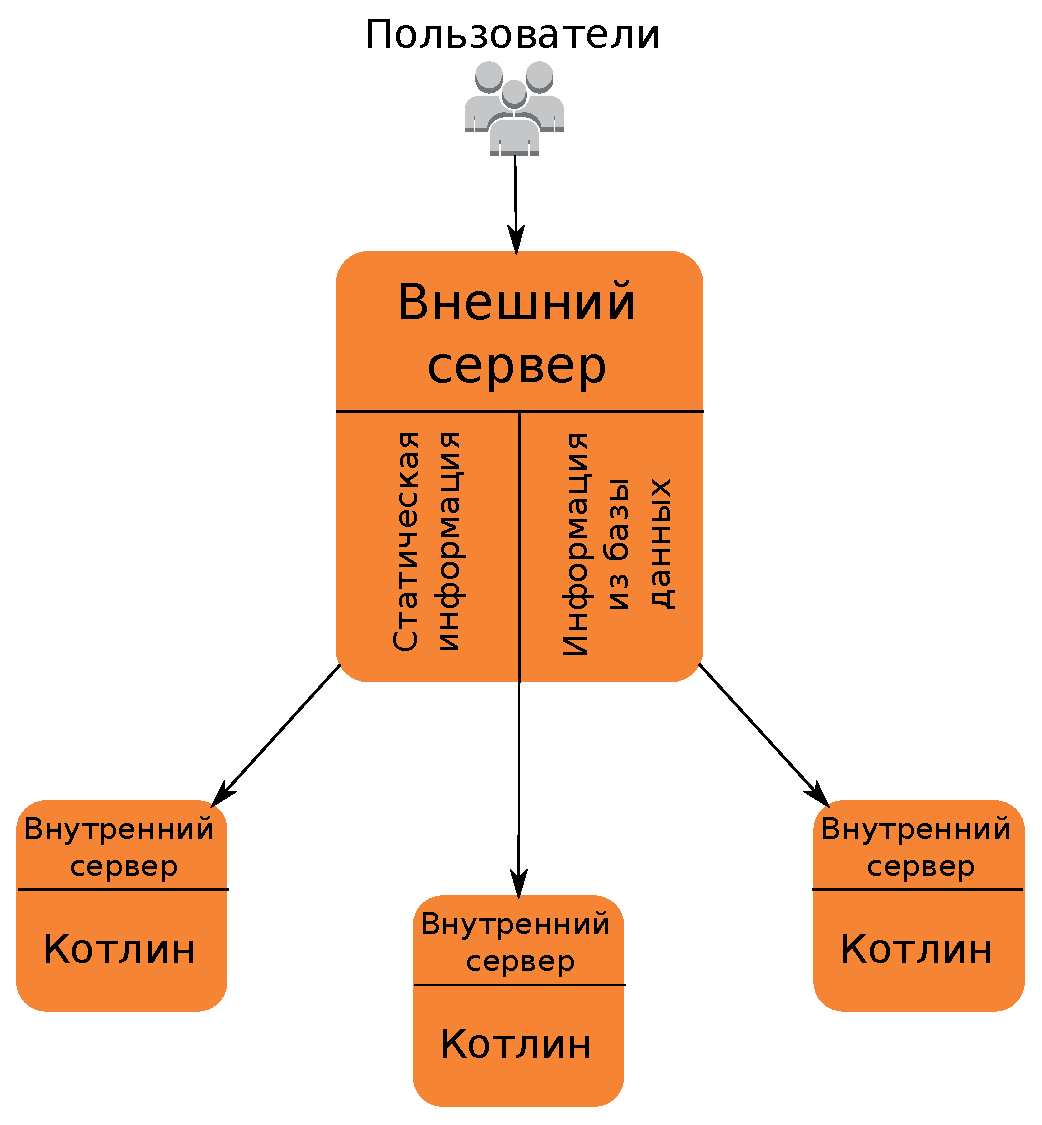
\includegraphics[scale=0.8]{app_schema}
	\end{center}
	\caption{Устройство серверной части приложения}
\end{figure}	


\section{База данных}
	В данном проекте используются две базы данных, схемы которых приведены в приложении \ref{}. Обе используются исключительно внешним сервером.
	
	Первая база данных -- это база данных приложения, в ней хранится информация о пользовательских проектах. Данная база состоит из трёх таблиц -- таблицы с пользователями, таблицы с проектами и таблицы с файлами. Каждый проект имеет ссылку на автора, каждый файл имеет ссылку на проект, к которому он принадлежит. 
Во всех трёх таблицах помимо первичных ключей, которые используются только внутри базы, имеются дополнительные ключи, которые используются в HTTP-запросах.
	
	Вторая база данных используется внешним сервером для хранения информации о HTTP-сессииях. Такой подход к хранению сессий позволяет разделять эту информацию между различными серверами и, благодаря этому, не терять её при обновлении приложения (см. главу \ref{}). 

	
	%Написать про базу данных
	%Добавить картинку
	%Обновление бэкенда при обновлении версии Котлина
	%Сказать про JS конфигурацию
\section{Внешний сервер}
	Внешний сервер принимает все запросы, приходящие от пользователя. Эти запросы делятся на несколько типов:
\begin{itemize}
	\item Запросы, обрабатываемые на внешнем сервере
	\item Запросы  к базе данных
	\item Запросы к внутренним серверам
\end{itemize}

	Запросы, обрабатываемые на внешнем сервере, это, в основном, запросы на получение статических данных. К этим данным, в первую очередь, относится вся клиентская часть кода в виде HTML/CSS/JavaScript файлов. Также к статическим данным относятся примеры, хранящиеся на внешнем сервере.
	
	%TODO: проверка синтаксиса считает, что можно "авторизоваться", но не "авторизироваться". Поправь ранее
	%TODO: Авторизоваться = залогинться = войти в свою учётную запись = войти в свой профиль, сделай что-нибудь с этим адом лексических повторов
	Кроме запросов на получение статических данных, внешний сервер обрабатывает запросы на авторизацию. Поскольку в данном приложении отсутствует встроенный механизм авторизации, то все эти запросы перенаправляются на сайт другого сервиса, позволяющего пользователю авторизоваться. Если авторизация прошла успешно, то сервис авторизации возвращает всю интересующую нас информацию, в нашем случае -- идентификатор пользователя и его имя. На данный момент авторизоваться можно через сервисы google, facebook, twitter, github или JetBrains. Во всех случаях, кроме сервиса JetBrains, для авторизации используется протокол OAuth.
	
	
	При успешной авторизации информация о пользователе записывается внутрь HTTP-сессии и, если пользователь заходит впервые, заносится в базу данных.
	
	
	Запросы к базе данных отправляются только для авторизованных пользователей. Данные запросы позволяют выполнять все необходимые операции с пользовательскими проектами и файлами(получить, создать, обновить, удалить)).
	
	%TODO: проверь, что все "в течении" -> "в течение". Т.к. ты работаешь с промежутками времени, а не с рекой воды
	Все запросы, связанные с Котлином, пересылаются внутренним серверам, после чего в течение определённого времени ожидается ответ, который отправляется обратно пользователю. Если же ответ не приходит, то пользователю отправляется соответствующее сообщение об ошибке.
	
	

\section{Внутренний сервер}
	Как уже было сказано в предыдущей главе, внутренний
сервер обрабатывает запросы, связанные с Котлином. Эти запросы делятся на 5 типов:
\begin{itemize}
	\item Запросы на получение списка ошибок в коде
	\item Запросы на автодополнение
	\item Запросы на конвертацию кода на языке Java в код на языке Котлин
	\item Запросы на трансляцию кода на языке  Котлин в код на языке JavaScript.
	\item Запросы на исполнение кода на языке Котлин.
\end{itemize}
	Для обработки этих запросов на внутреннем сервере используется последняя версия библиотек Котлина. Обработка всех запросов, кроме запросов на исполнение программ, в итоге сводится к вызову методов из этих библиотек. Такой подход является наиболее простым, однако у него есть один недостаток -- мы не можем ограничить время исполнения вызванного метода, а значит и время обработки запроса. Это связано с тем, что поток в языке Java не может быть завершён извне. 
	
	%TODO: любишь писать "и.т.д." вместо "и т.д."
	При обработке запроса на исполнение сначала, при помощи библиотек Котлина, код компилируется в байткод JVM. Далее скомпилированный код исполняется в отдельном процессе внутри класса-обёртки. В целях безопасности	процесс, в котором исполняется пользовательская программа, ограничен по памяти (Xmx настройка java-машины), ограничен по времени исполнения (через 5 секунд процесс завершается из сервера), а также ему запрещён доступ к сети, файловой системе и т.д. при помощи Java security manager. 
	
	В случае JVM конфигурации класс-обёртка, используя reflection, запускает функцию main в пользовательском коде, то есть просто исполняет пользовательскую программу. При этом весь вывод программы (System.out, System.err) перенаправляется в форматированном виде в один поток. Если внутри пользовательского кода происходит исключение, то оно ловится классом-обёрткой. По завершении пользовательской программы весь вывод, а также исключение (если есть), сериализуются в формат JSON и полученная строчка выводится в стандартный вывод класса-обёртки.
	
	%TODO: "по завершению" -> "по завершении" исправь, где найдёшь ещё.
	В случае Junit конфигурации, используя встроенные средства этой библиотеки, запускаются все тестовые методы, найденные внутри пользовательских классов. При запуске каждого теста сохраняется вывод программы и ошибки, вылетевшие в процессе исполнения. По завершении исполнения всех тестов эта информация так же сериализуется в формат JSON и выводится в стандартный поток вывода.
	

	
	
	

\chapter{Инфраструктура}

В данной главе подробно рассмотрены детали масштабируемой архитектуры приложения.

\section{Внутренние сервера}
\subsection{Старт нового сервера}
	При автоматическом запуске машины на Amazon мы можем передать очень маленькое количество информации, а именно, идентификатор AMI и User Data - небольшой набор инструкций, который будет выполнен после запуска. Данный параграф посвящён тому, как при помощи этого небольшого количества данных можно настроить компьютер и запустить приложение.
	
	Для того, чтобы просто запустить компьютер нам достаточно идентификатора AMI. Первоначально нами был выбран образ с CoreOS, т.к. планировалось запускать приложение внутри докер-контейнера, а CoreOS как раз предназначена для таких случаев.
	
	После того, как мы запустили компьютер нам необходимо скачать наше приложение и всю необходимую инфраструктуру, используя при этом только докер, т.к. в CoreOS кроме него ничего нет.
	
	Теоретически, всё приложение вместе с инфраструктурой можно было бы поместить внутрь одного докер образа, а при старте машины запустить докер-контейнер, основанный на нём. Проблема такого подхода заключается в том, что при обновлении исходного кода приложения, что происходит очень часто, нам приходилось бы добавлять слой, что приводило бы к сильному росту размера образа.
	
	С учётом этого был применён несколько другой подход, при котором вся необходимая инфраструктура и настройки, которые меняются достаточно редко, помещаются в докер образ, а само приложение хранится в S3Bucket - облачном хранилище Amazon. В такой ситуации при старте машины нам необходимо  скачать наше приложение из S3 при помощи соответствующего приложения, запущенного внутри докер контейнера. После этого мы можем запускать основной контейнер, который основывается на образе с настройками, и передать ему скачанное приложение.
	
	Все необходимые докер-контейнеры запускаются в виде системного сервиса (см. systemd). Это позволяет сохранить информацию об ошибках, возникших при исполнении контейнеров. Также при таком подходе контейнер с приложением может быть автоматически перезапущен в случае если его исполнение завершилось с ошибкой.
	
	В результате получается следующая User Data:
\begin{lstlisting}
[Unit]
Description=Kotlin web Demo backend Green
After=docker.service

[Service]
TimeoutStartSec=1800s
Restart=always
ExecStartPre=-/usr/bin/docker rm -f war-container-green
ExecStartPre=/usr/bin/docker run --name=war-container-green -v /wars docker-registry.labs.intellij.net/itops/aws-cli s3 cp s3://kotlin-web-demo-backend/green/WebDemoBackend.war /wars
ExecStartPre=/usr/bin/docker pull docker-registry.labs.intellij.net/kotlin/web-demo-backend
ExecStart=/usr/bin/docker run -m="1536m" --rm=true -e "LFS_NAME=kotlin.web.demo.backend" --name tomcat-green --volumes-from war-container-green -p 8080:20039 docker-registry.labs.intellij.net/kotlin/web-demo-backend

ExecStop=/usr/bin/docker stop tomcat-green
\end{lstlisting}

\subsection{Выбор типа компьютера}
	%TODO: всюду "тип"
	Одним из параметров конфигурации запуска компьютера на Amazon является его тип. Он определяет то, насколько мощный будет CPU, количество памяти и.т.д.. Также от него зависит стоимость -- чем лучше параметры, тем дороже компьютер стоит, что делает выбор типа компьютера важным этапом создания инфраструктуры на Amazon.
	
	В таблице \ref{table:instance_types} приведены основные характеристики тех типов, которые рассматривались в качестве кандидатов.
	
	Как видно, CPU у ряда типов компьютеров, а именно, у компьютеров типа t2, помечены Burstable. Это -- возможность временно увеличивать производительность CPU, тратя при этом кредиты CPU. Кредиты CPU -- это абстракция, использующаяся Amazon. Они копятся со временем и теряются либо при большом потреблении CPU, либо по истечении суток. Подобная система разработана для приложений, у которых в среднем нагрузка мала, однако периодически она может возрастать.
	
\begin{table}[h]
	\centering
	\begin{tabular}{l|c|c|c}
		Type      & CPU Units    & Memory & Cost\\ \hline
		t2.small  & 1(Burstable) & 2GB    & \$0.026 hourly\\ \hline
		t2.medium & 2(Burstable) & 4GB    & \$0.052 hourly\\ \hline
		m3.medium & 3            & 3.75GB & \$0.070 hourly\\ \hline
		c4.large  & 8            & 3.75GB & \$0.116 hourly\\
	\end{tabular}
	\caption{Параметры интересующих нас типов амазоновских инстансов}
	\label{table:instance_types}
\end{table}
	
	Для сравнения производительности компьютеров использовались два простых нагрузочных теста. В обоих тестах на сервер посылались запросы на исполнение ``Hello, World!'' программы. В первом случае запросы постоянно отправлялись из одного потока, и измерялось время обработки каждого запроса. Во втором случае измерялось максимальное количество потоков, при котором сервер успевал исполнять программу (через 5 секунд после старта программа завершается).
	
\begin{table}[h]
	\centering
	\begin{tabular}{l|c|c}
		Type      & Время обработки запроса    & Максимальное число потоков\\ \hline
		t2.small  & 0.5(Burst)/2.5             & 7(Burst)/1  \\ \hline
		t2.medium & 0.5(Burst)/2.5             & 15(Burst)/2 \\ \hline
		m3.medium & 1.2                        & 4           \\ \hline
		c4.large  & 0.5                        & 10          \\
	\end{tabular}
	\caption{Параметры интересующих нас типов амазоновских инстансов}
	\label{table:instance_types_performance}
\end{table}

	Из двух приведённых выше таблиц видно, что нам явно не подходят m3.medium инстансы, т.к. у них стабильно низкая мощность CPU.
	
	Намного интересней всё с компьютерами типа t2. Из таблицы \ref{table:instance_types_performance}	 видно, что они могут выдавать производительность даже большую, чем более дорогие компьютеры типа c4.large, но есть очевидная проблема, которая заключается в том, что мы можем потратить все CPU кредиты. Данная проблема наиболее существенна при возникновении достаточно долгой большой нагрузки, т.к. общего числа накопленных кредитов может хватить максимум на час работы при максимальном потреблении CPU. В такой ситуации один компьютер перестанет справляться, и система автоматического масштабирования должна будет поднять новые, которые тоже будут типа t2. А это означает, что каждая поднятая машина в таких условиях сможет нормально работать только в течение часа, после чего она станет почти бесполезной. 
	
	Также существует ещё одна связанная с кредитами проблема. Ресурсом, который мы активней всего тратим, является CPU, поэтому и наши метрики, которые отвечают за масштабирование, настроены на то, чтобы смотреть на потребление CPU. Когда у t2 компьютера кончаются кредиты уровень потребления CPU у него не поднимается выше 20\%. Это приводит к тому, что согласно нашим метрикам, нагрузка на систему мала, а значит и новые компьютеры поднимать не нужно. Данная ситуация является катастрофичной, т.к. сервера не смогут обрабатывать запросы в связи с тем, что они перегружены, а система масштабирования будет считать что всё нормально и ничего не предпринимать, что приведёт к неработоспособности приложения до тех пор, пока не спадёт нагрузка.
	
	Учитывая всё вышесказанное, можно сказать, что компьютеры типа t2 обладают очень хорошим соотношением мощности к цене, однако в сколь бы то ни было серьёзном приложении их использование представляется невозможным в связи с непредсказуемостью поведения. Учитывая это, а так же тот факт , что тип m3.medium обладает очень слабым процессором, в итоге были выбран тип компьютеров с4.large.
\subsection{Подбор метрик}
	Как было сказано ранее, автоматическое масштабирование в амазоне основано на событиях Cloud Watch Alarm, каждое из которых говорит о том, что потребление определённого ресурса было больше/меньше определённого уровня.
	
	%TODO: либо "учитывая это, мы сделали ...", либо "с учётом этого было сделано ... "
	Как показал мониторинг нашего приложения, ресурс, который мы можем целиком потратить, один - процессорное время. С учётом этого были созданы соответствующие события:
\begin{itemize}
	\item Если среднее потребление CPU больше 80\% в течение 2 минут, то увеличить количество инстансов в 2 раза, после чего подождать одну минуту перед следующим масштабированием.
	\item Если среднее потребление CPU меньше 40\% в течение часа, то 
\end{itemize}

	При срабатывании первого события система атвоматического масштабирования должна увеличить количество компьютеров в 2 раза, после чего в течение минуты не предпринимать никакой активности.
	
	При срабатывании второго события система должна уменьшить количество компьютеров на 1, после чего подождать пять минут перед следующим масштабированием.

	Из предыдущих абзацев видно, что существенно различается время, которое мы ждём, перед тем как запускать новые компьютеры и перед тем как уничтожать старые. Это позволяет нам избежать ситуации, при которой мы будем останавливать только что запущенные компьютеры из-за того, что немного уменьшилась нагрузка, а потом запускать их обратно, т.к. нагрузка обратно возросла. Кроме того, при старте новой машины на амазоне мы оплачиваем один час её работы, что делает подобный подход ещё более осмысленным.
	
	Выбранная нами политика масштабирования является очень агрессивной, т.е. она очень мало ждёт перед поднятием новых компьютеров и увеличивает их количество в геометрической прогрессии. Это сделано для того, чтобы мы могли оперативно среагировать на резко увеличившуюся нагрузку. Недостатком такого подхода является то, что при случайном превышении порога, мы можем поднять много лишних машин, но в случае нашего приложения этот недостаток не проявляется, т.к. средняя нагрузка на наше приложение сильно меньше порога.
	
\subsection{Время запуска машины. Использование AMI}
	Время отклика приложения на рост нагрузки зависит не только от того, как мы настроили события в Cloud Watch, но и от того, как долго будет запускаться новый компьютер и сколько времени будет настраиваться на нём наша инфраструктура. 
	
	Со временем запуска новой машины мы сделать ничего не можем, это время более-менее постоянно и равно 1-2 минутам, а вот время настройки инфраструктуры мы можем пытаться уменьшить. В первоначальной версии это время составляло порядка 7 минут, что приводило к тому, что суммарное время отклика на рост нагрузки было больше 10 минут (2 минуты для срабатывания события, 2 минуты чтобы запустить машину, 7 минут чтобы настроить инфраструктуру). Основную часть этого времени мы тратили на скачивание образов докера, среди которых есть очень объёмный образ операционной системы.
	
	Единственный способ избежать скачивания докер-образов -- это иметь эти докер образы локально. Это можно сделать, если создать образ работающей машины и использовать его для запуска новых машин. При таком подходе время настройки нашей инфраструктуры удалось сократить до нескольких минут, что привело к суммарному времени порядка 5 минут. 
\section{Инфраструктура с учётом обновлений}
\subsection{Green Blue deployment}
	Среди многочисленных подходов к тому, как обновлять приложение, нами был выбран ``Blue Green Deployment'', при котором существует две версии приложения, одна из которых является активной. Схема данного подхода в случае нашего приложения приведена на рис.\ref{fig:green_blue_deployment}.
\begin{figure}[h]
    \centering
    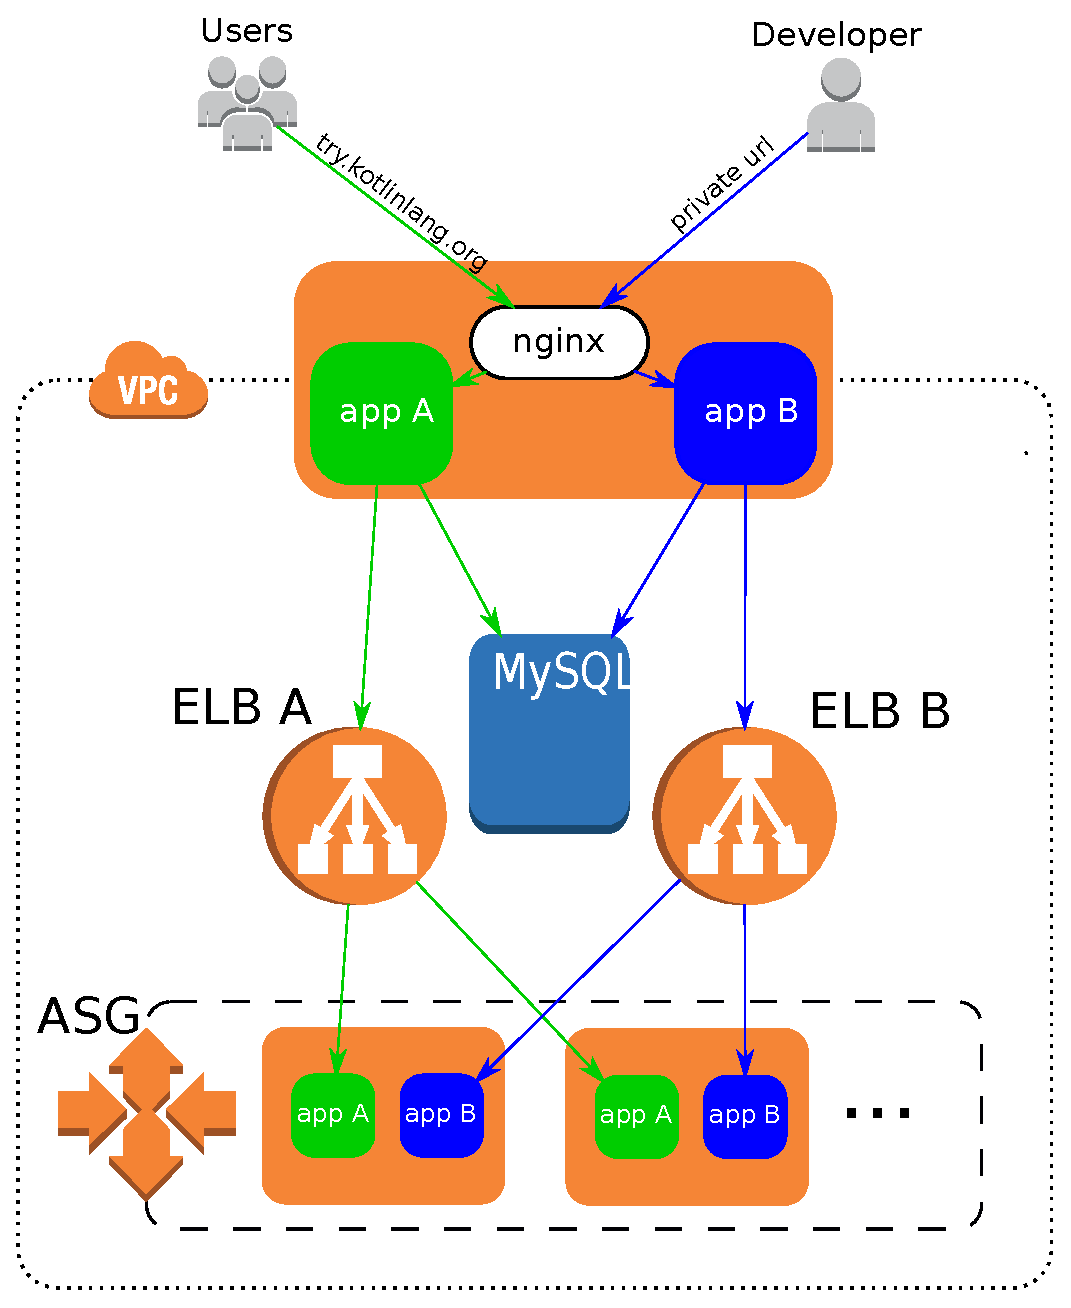
\includegraphics[scale=0.8]{green_blue_deployment} 
    \caption{Детальная схема устройства нашего приложения. Зелёным отмечено активное приложение, синим -- пассивное}
    \label{fig:green_blue_deployment}
\end{figure}

	Какое приложение является на данный момент активным определяется в нашей схеме настройками nginx сервера, который принимает все запросы извне. Если запрос был отправлен на публичный адрес try.kotlinlang.org, то он будет перенаправлен активному приложению, а если он был отправлен на адрес, который известен только разработчикам, то он будет перенаправлен в пассивную ветку приложения.
	
	При публикации приложения оно сперва выкладывается в пассивную ветку, после чего проверяется его работоспособность. Если приложение работоспособно, то далее меняются настройки nginx-сервера  и обновлённое приложение становится активным, что завершает процесс публикации обновлений.
\subsection{Выбор стоимость-надёжность}
	Как видно из рисунка .\ref{fig:green_blue_deployment}, мы не дублируем никакие машины кроме ELB, которые необходимо дублировать, т.к. они умеют слушать только один порт и отправлять запросы тоже только на один порт. Такая схема является экономной, однако имеет свои недостатки.
	
	Основным минусом такой схемы является то, что при возникновении проблем в обновлённой версии приложения могут возникнуть проблемы в активном приложении.
	
	На внешнем сервере подобной проблемы нет, т.к. каждое из приложений работает внутри своего докер-контейнера, и если в одном из них происходит ошибка, то второе ничего не замечает, т.к. они работают в изолированном окружении.
	
	На внутренних серверах всё было бы точно так же, если бы внутренние сервера не проверялись постоянно на работоспособность балансировщиком нагрузки. Это приводит к тому, что если одно из наших приложений не отвечает по какой-то причине (что-то зависло в процессе публикации, мы выложили плохое приложение и.т.д), то данный компьютер будет остановлен, а на смену ему будет поднят новый. В худшем случае с новым компьютером всё может повториться и система автоматического масштабирования так и будет запускать и останавливать новые компьютеры, пока мы не починим приложение.
	
	Самым простым решением данной проблемы является копирование инфраструктуры для пассивного приложения, но в такой ситуации нужно тратить дополнительные деньги на работу инстансов пассивной ветки.
\chapter{Тестирование}
\section{Тестирование серверного кода}
	Тестирование серверного кода является частью автоматической сборки приложения на TeamCity. Оно производится при помощи библиотеки JUnit. В процессе тестирования проверяется, что:
\begin{itemize}
\item Сервер корректно транслирует Java код в Котлин
\item Сервер корректно автоматически дополняет код
\item Сервер корректно обнаруживает ошибки в коде.
\item Сервер корректно исполняет код.
\item Сервер выдаёт ошибки при исполнении небезопасного кода.
\item В примерах не содержится ошибок. 
\end{itemize}
	
	Основным преимуществом такого набора тестов является возможность безопасного обновления версии Kotlin, использующуюся для обработки пользовательских запросов. Также данные тесты проверяют корректность работы приложения при изменении серверного кода.
	
	Для проверки корректности примеров каждый из них подвергается ряду тестов. Во-первых, код примера проверяется сервером на наличие ошибок и предупреждений. Если сервер находит какие-либо ошибки, то это означает, что наш пример не компилируется новой версией Kotlin, и что этот пример необходимо обновить. Во-вторых, проверяется, что данный пример компилируется и при запуске выдаёт ожидаемый результат. Следует отметить, что такие тесты проверяют не только примеры, но и работоспособность самого сервера (его возможность запускать проекты и находить ошибки). 
	
	Кроме примеров существует ещё ряд тестовых программ, которые  используются для тестирования. При их помощи проверяется ряд особых случаев (использование Kotlin reflection, например), а также корректность реакции на код, который пытается выполнить небезопасные действия (доступ к файловой системе, к сети и т.д.).
	
\section{Нагрузочное тестирование}

	Нагрузочное тестирование интернет-приложения~--- это проверка его поведения при большом количестве запросов. Такое тестирование позволяет выявить проблемы, возникающие при этом, и оценить максимальное количество пользователей, которое может обслужить данное приложение.
	
	В случае нашего приложения ожидаемым узким местом были запросы на исполнение программы. В рамках нагрузочного тестирования планировалось: 
\begin{itemize}
\item Проверить сервер на наличие других узких мест.
\item Проверить поведение сервера при исполнении особых программ, а именно:
	\begin{itemize}
		\item Исполнение бесконечных программ
		\item Исполнение программ, потребляющих бесконечное количество памяти
		\item Исполнение программ, генерирующих бесконечно большой вывод.
	\end{itemize}
\item Проверить работоспособность автоматического масштабирования
\item Узнать количество пользователей, которых может обслужить одина виртуальная машина внутреннего сервера.
\item Посмотреть на поведение внутреннего сервера при подаче на него большой нагрузки
\end{itemize}

	Нагрузочное тестирование проводилось при помощи программы Jmeter.

	Чтобы проверить сервер на наличие узких мест использовался тот факт, что запросы делятся на несколько типов. Сервер нагружался запросами одного типа, и исследовалось его поведение. Так, например, для проверки внешнего сервера отправлялись запросы на выдачу статического контента и запросы на выдачу примеров.
	
	В результате таких проверок внешнего сервера получились следующие параметры:
\begin{itemize}
	\item 9 заходов новых пользователей в секунду (т.е. 32000 новых заходов в час) (~200MiB/s bandwidth out)
	\item 700 запросов на загрузку примера в секунду
\end{itemize}
	Данные параметры являются вполне приемлемыми для нашего приложения, а значит, внешний сервер не является узким местом приложения. 
	
	Ещё одним потенциально узким местом приложения является база данных, но, согласно статистике использования нашего приложения, большинство пользователей не авторизуются, а значит и запросы к базе данных не отправляют.
	
	Это означает, что единственным узким местом нашего приложения являются внутренние сервера, поэтому при оценке производительности системы рассматривались исключительно запросы к внутреннему серверу.

	Для того, чтобы оценить количество пользователей, которое может обслужить наше приложение, необходимо было составить модель поведения пользователя. Это было сделано на основе сохранённых записей об активности пользователей на старом сайте kotlin-demo.jetbrains.com. В результате были созданы две модели пользователя:
\begin{itemize}
	\item Активный пользователь~--- 13 запросов на проверку ошибок в минуту, 1 запрос на автодополнение в минуту, 1 запрос на исполнение в минуту.
	\item Усреднённый пользователь~--- 4 запроса на проверку ошибок в минуту, 1 запрос на автодополнение в три минуты, 1 запрос на исполнение в три минуты.
\end{itemize}
	
	В результате нагрузочного тестирования внутренних серверов были получены следующие результаты:
	\begin{itemize}
		\item Одна машина:
		\begin{itemize}
			\item максимум 2.75 запросов на исполнение в секунду;
			\item максимум 110 ``активных'' пользователей
			\item максимум 370 ``усреднённых'' пользователей
		\end{itemize}
		
		\item Предельная нагрузка на всю систему, приблизительная, при 10 запущенных машинах:
		\begin{itemize}
			\item 3500-4000 пользователей
		\end{itemize} 
	\end{itemize}
	Также был обнаружен ряд проблем с памятью, возникающих при исполнении программ, генерирующих бесконечный вывод. Впоследствии данные проблемы были устранены путём введения ограничений на потребляемую память для пользовательских процессов, сервера, а также докер-контейнера, в котором всё исполняется.
	
\section{Тестирование клиентского кода}
	Тестирование клиентского кода является важной частью тестирования и при этом, пожалуй, наиболее сложной частью. Сложность подобного тестирования заключается в том, что
\begin{enumerate}
	\item  Для тестирования клиентского кода необходим запущенный сервер или его имитация.
	\item Клиентский код исполняется в браузере, причём в разных браузерах может наблюдаться  различное исполнение кода.
	\item Для полноценного тестирования необходимо тестировать не только код, но и внешний вид приложения и проверять, что он не отличается в различных браузерах.
\end{enumerate}

	На данный момент описанные выше проблемы, по большому счёту, не решены. Имеющееся тестирование клиентского кода заключается в небольшом наборе selenium тестов, которые проверяют корректность подсветки кода, корректность исполнения программ, а также работу с проектами. Данные тесты требуют запущенного сервера и запускаются внутри браузера firefox, что делает невозможным их запуск в процессе автоматической сборки приложения.
	
	В связи с недостатками имеющегося тестирования и, учитывая описанные выше сложности тестирования клиентского кода, сейчас разрабатывается новая система тестов. 
Основой данной системы тестов является программа karma, которая позволяет запускать тесты в различных средах. Это сделает возможным запуск тестов на любой машине, т.к. отпадает требование наличия конкретного браузера. Одной из возможных сред является phantomjs, что позволяет запускать тесты на машинах без браузеров вообще, в том числе на агентах сервера сборки приложений. 
	
	
\chapter*{Заключение}
\addcontentsline{toc}{chapter}{Заключение}
	В рамках данной работы была создана новая версия онлайн-среды разработки для языка Котлин. По сравнению с предыдущей версией, новое приложение обладает следующими преимуществами:
\begin{itemize}
	\item Поддержка многофайловых проектов
	\item Поддержка JUnit тестов
	\item Масштабируемая архитектура
\end{itemize}
	
	Масштабируемая часть приложения была протестирована. В рамках тестирования было оценено максимальное число пользователей, а также время восстановления системы после перегрузки.
	
	Была разработана инфраструктура (см. главу\ref{ch:infrastructure}), позволяющая обновить приложение при изменении его исходного кода, настроек приложения или требований к окружению. Данная схема обладает следующими преимуществами:
	
\begin{itemize}
	\item Возможность проверки работоспособности обновлённого приложения перед его публикацией
	\item Возможность обновления приложения без остановки его работы.
	\item Резервная версия приложения, которая может быть использована в случае выхода основной версии из строя.
\end{itemize}

	Был автоматизирован процесс настройки окружения, а также процессы публикации приложения и его обновления.
	
\section*{Направления развития}

	В дальнейшем планируется использовать данное приложение в качестве платформы для обучения языку Котлин. Для этого будет использован имеющийся набор задач, который будет транслирован в набор проектов для Web Demo. На данный момент эти задачи представлены в виде проекта для IntellijIdea. По мере выполнения пользователем данных задач он сможет наблюдать свой прогресс.
	
	Также важным направлением развития является встраиваемость приложения в другие web-страницы. Одним из примеров использования встраиваемого приложения является публикация новостей о Котлине. При этом, как правило, выкладываются примеры кода, которые демонстрируют изменения языка. Данные примеры можно сделать исполняемыми, что позволит пользователю посмотреть на нововведения, не переходя при этом на сайт онлайн-среды разработки.
\addcontentsline{toc}{chapter}{Литература}
\begin{thebibliography}{99}
    
    \bibitem{cloud_book}
	Thomas A. Limoncelli, Strata R. Chalup, Christina J. Hogan
    ``The Practice of Cloud
System Administration''

    \bibitem{project_kotlin}
    Project Kotlin http://kotlinlang.org/.
    
    \bibitem{tomcat}
    Tomcat server http://tomcat.apache.org/
    
    \bibitem{aws}
    Amazon Web Servivices  http://aws.amazon.com/documentation/
    
    \bibitem{docker}
    Docker https://www.docker.com/
    
    
    
    \bibitem{jquery}
    JQuery http://jquery.com/
    
    \bibitem{jqueryui}
    JQueryUI http://jqueryui.com/
    
    \bibitem{codemirror}
    CodeMirror http://codemirror.net/
    
    \bibitem{nodejs}
    NodeJS https://nodejs.org/
    
    \bibitem{karma}
    Karma http://karma-runner.github.io/
    
    \bibitem{junit}
    JUnit http://junit.org/


\end{thebibliography}

\chapter*{Благодарности}
В рамках данной работы я хотел бы выразить благодароность:
\begin{itemize}
	\item Андрею Бреславу за руководство моим проектом
	\item Сергею Жукову за помощь в создании масштабируемой инфраструктуры
	\item Роману Колобову за помощь в организации нагрузочного тестирования
	\item Антонине Весне за создание дизайна
	\item Залиму Башорову за интерес, проявленный к моей работе и содержательные комментарии
	\item Михаилу Глухих за помощь в составлении дипломной работы
	\item Команде JetBrains за уютную атмосферу
\end{itemize}

\end{document}
